\documentclass[a4paper,12pt]{scrartcl}
\usepackage[utf8]{inputenc}
\usepackage[ngerman]{babel}
\usepackage[T1]{fontenc}
\usepackage{amsmath}
\usepackage{stmaryrd}
\usepackage{wasysym}
\usepackage{lmodern}
\usepackage{graphicx}
\usepackage{paralist}
\usepackage{upgreek}
\usepackage{subfigure}
\usepackage{tipa}
\usepackage{amssymb}
\usepackage{gensymb}
\usepackage{dsfont}
\usepackage{mathtools}
\usepackage{ stmaryrd }
\usepackage{fancyhdr}

%\title{Abgabe 1}
%\author{Rafael Heid, Julian Deinert, Sabrina Buczko Gruppe\\ 6 und 7}
%\date{Abgabe am 24.10.16}

\gdef\blatt{FGI-2 Aufgabenblatt 06}

\title{\blatt}
\date{Gruppe 06}
\author{Sabrina Buczko 6663234, Julian Deinert 6535880, Rafael Heid 6704828}


\pagestyle{fancy}
\fancyhf{}
\fancyhead[L]{\blatt}
\fancyhead[R]{Buczko, Deinert, Heid}
\fancyfoot[C]{\thepage}

\begin{document}
\maketitle
\newpage
\setcounter{section}{5}
% Section 6
\section{}
\setcounter{subsection}{2}
% Section 6.3
\subsection{}
% Section 6.3.1
\subsubsection{}
\begin{tabular}{llll}
$VC(\phi_{01})=(1,0,0,0)$&$VC(\phi_{11})=(1,1,0,0)$&$VC(\phi_{21})=(0,0,1,0)$&$VC(\phi_{31})=(0,0,0,1)$\\
$VC(\phi_{02})=(2,0,0,0)$&$VC(\phi_{12})=(1,2,1,0)$&$VC(\phi_{22})=(0,0,2,1)$&$VC(\phi_{32})=(2,0,0,2)$\\
$VC(\phi_{03})=(3,3,1,0)$&$VC(\phi_{13})=(1,3,1,0)$&$VC(\phi_{23})=(2,0,3,3)$&$VC(\phi_{33})=(2,0,0,3)$\\
$VC(\phi_{04})=(4,3,1,4)$&$VC(\phi_{14})=(1,4,1,0)$&$VC(\phi_{24})=(5,3,4,4)$&$VC(\phi_{34})=(2,0,0,4)$\\
$VC(\phi_{05})=(5,3,1,4)$&$VC(\phi_{15})=(5,5,5,4)$&$VC(\phi_{25})=(5,3,5,4)$&$VC(\phi_{35})=(2,4,1,5)$\\
$VC(\phi_{06})=(6,3,1,4)$&$VC(\phi_{16})=(5,6,5,6)$&$VC(\phi_{26})=(6,3,6,4)$&$VC(\phi_{36})=(2,4,1,6)$\\
\end{tabular}
% Section 6.3.2
\subsubsection{}
Bei den Ereignissen $\phi_{34}, \phi_{04}, \phi_{24}$ und $\phi_{15}$ gilt\\
$\phi_{34}\ vor\ \phi_{04}\ vor\ \phi_{24}\ vor\ \phi_{15}$ mit\\
$(2,0,0,4)_{\phi_{34}} < (4,3,1,4)_{\phi_{04}} < (5,3,4,4)_{\phi_{24}} < (5,5,5,4)_{\phi_{15}}$.
% Section 6.3.3
\subsubsection{}
Die Ereignisse $\phi_{11}, \phi_{02}, \phi_{21}, \phi_{31}$ sind paarweise unabhängig:\\
$(1,1,0,0)_{\phi_{11}}\ ||\ (2,0,0,0)_{\phi_{02}}\ ||\ (0,0,1,0)_{\phi_{21}}\ ||\ (0,0,0,1)_{\phi_{31}}$.
% Section 6.3.4
\subsubsection{}
Die Ordnung der ersten Ereignisse gemäß Lamport-Ordnung sieht wie folgt aus:\\
$\phi_{01} <_L \phi_{21} <_L \phi_{31} <_L \phi_{02} <_L \phi_{11} <_L \phi_{22} <_L \phi_{12} <_L \phi_{32}$
% Section 6.3.5
\subsubsection{}
Der Präzedenzgraph ist praktisch bereits auf dem Zettel angegeben, fügt man an Stelle der ungerichteten Kanten der einzelnen Prozesse, nach rechts gerichtete Kanten ein.\\
Ich werde meine Zeit nicht darauf verwenden, einen vorhandenen Graphen nochmal zu zeichnen.
% Section 6.3.6
\subsubsection{}
Folgendes Petrinetz haben wir zu dem gegebenem Zeitskalenmodell angefertigt:\\
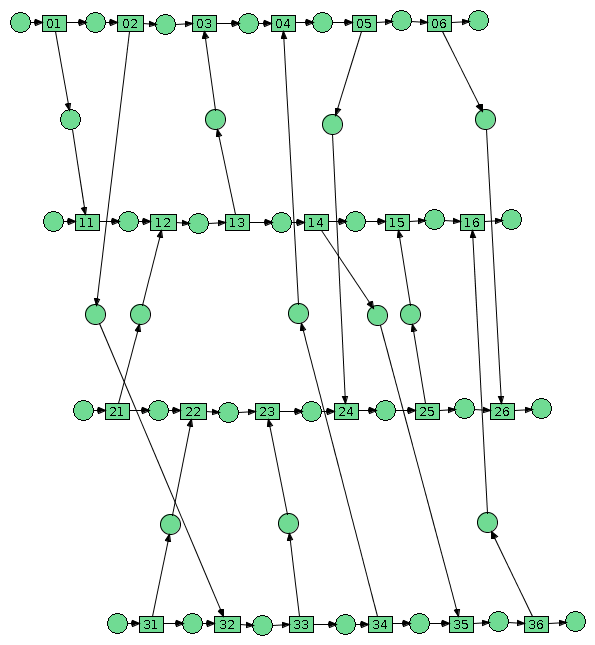
\includegraphics[scale=0.5]{./b06_a636.png}
% Section 6.4
\subsection{}

% Section 6.4.1
\subsubsection{}
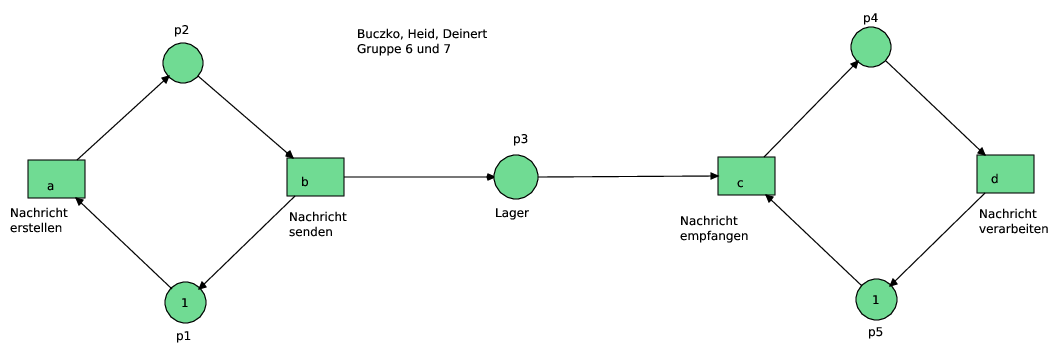
\includegraphics[scale=0.4]{6_4_1.png}

% Section 6.4.2
\subsubsection{}
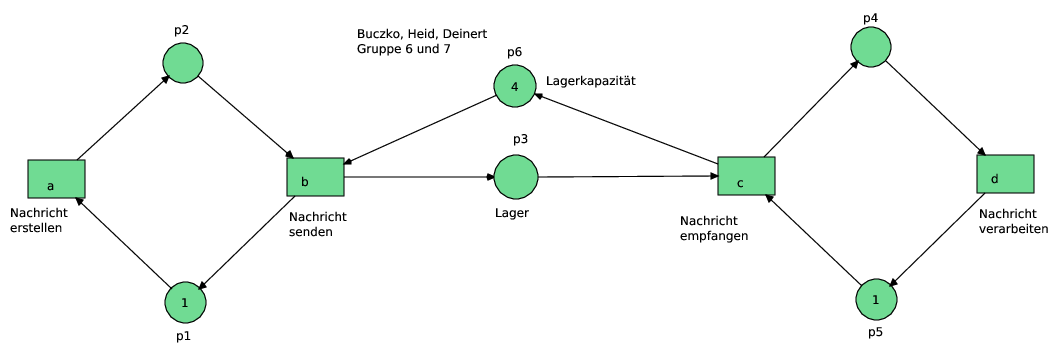
\includegraphics[scale=0.4]{6_4_2.png}
\\
Wir haben eine Lagerkapazitätsstelle $p6$ hinzugefügt. 
Auf dieser Stelle liegen initial 4 Marken. $b$ benötigt zum Schalten 
immer eine Marke auf $p6$. Wenn eine Nachricht empfangen wird, 
platziert $c$ wieder eine Marke auf $p6$.

% Section 6.4.3
\subsubsection{}
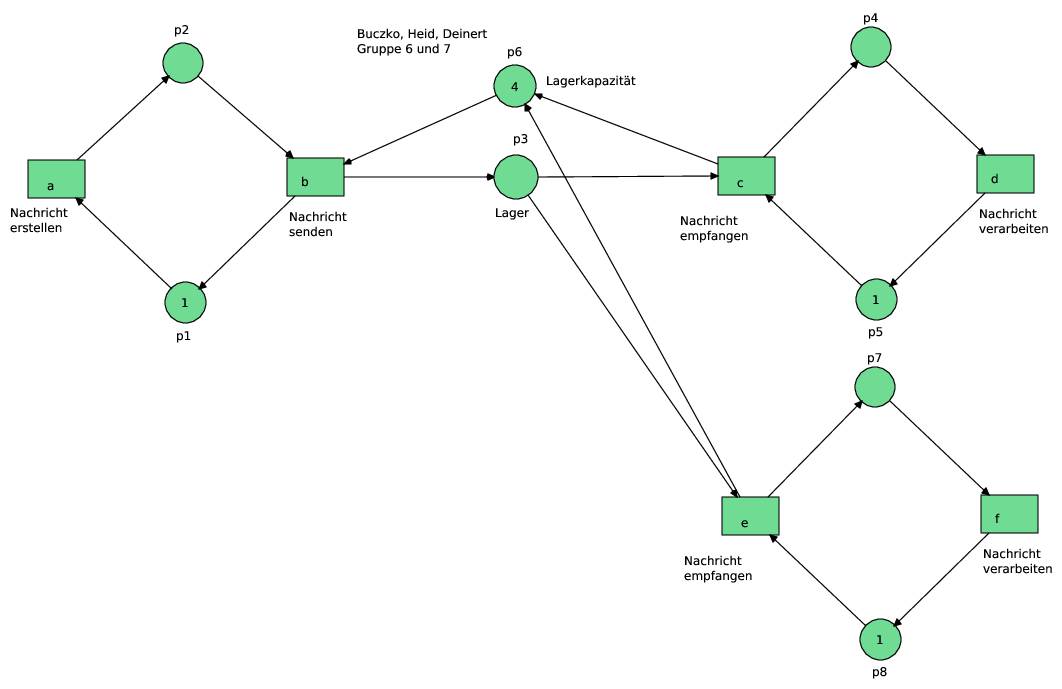
\includegraphics[scale=0.4]{6_4_3.png}
\\
Der zweite Empfänger entspricht exakt dem ersten und kann Nachrichten von $p3$ erhalten. Da in der Aufgabe nicht spezifiziert wurde, dass beide die selbe einzelne Nachricht erhalten können sollen, haben wir uns hier für die einfachere Implementation entschieden. 

% Section 6.4.4
\subsubsection{}
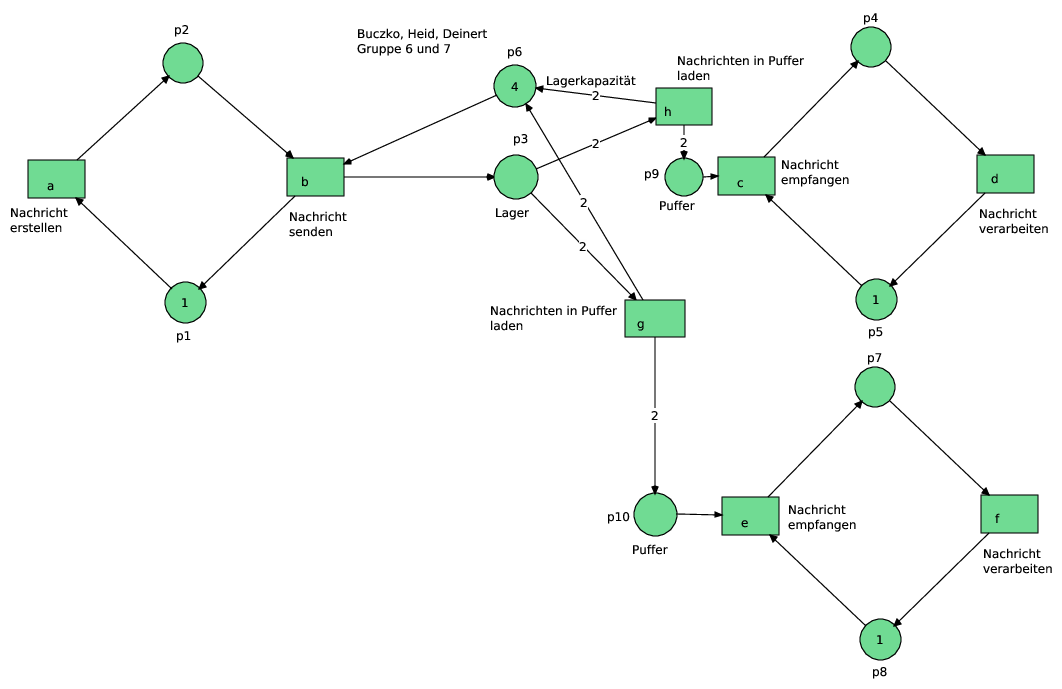
\includegraphics[scale=0.4]{6_4_4.png}
\\
Wir haben hierzu zwei Nachrichtenpuffer $p9$ und $p10$ sowei zwei 
Transitionen $h$ und $g$ erstellt, die die Nachrichten in den Puffer 
laden. Durch die Kantengewichte an den Ausgangskanten des Lagers, 
stellen wir sicher, dass immer genau zwei Nachrichten entnommen 
werden. Durch die Kantengewichte an den Kanten zur Lagerkapazität 
stellen wir sicher, dass immer wieder richtig viele Plätze frei 
werden. 

% Section 6.4.5
\subsubsection{}
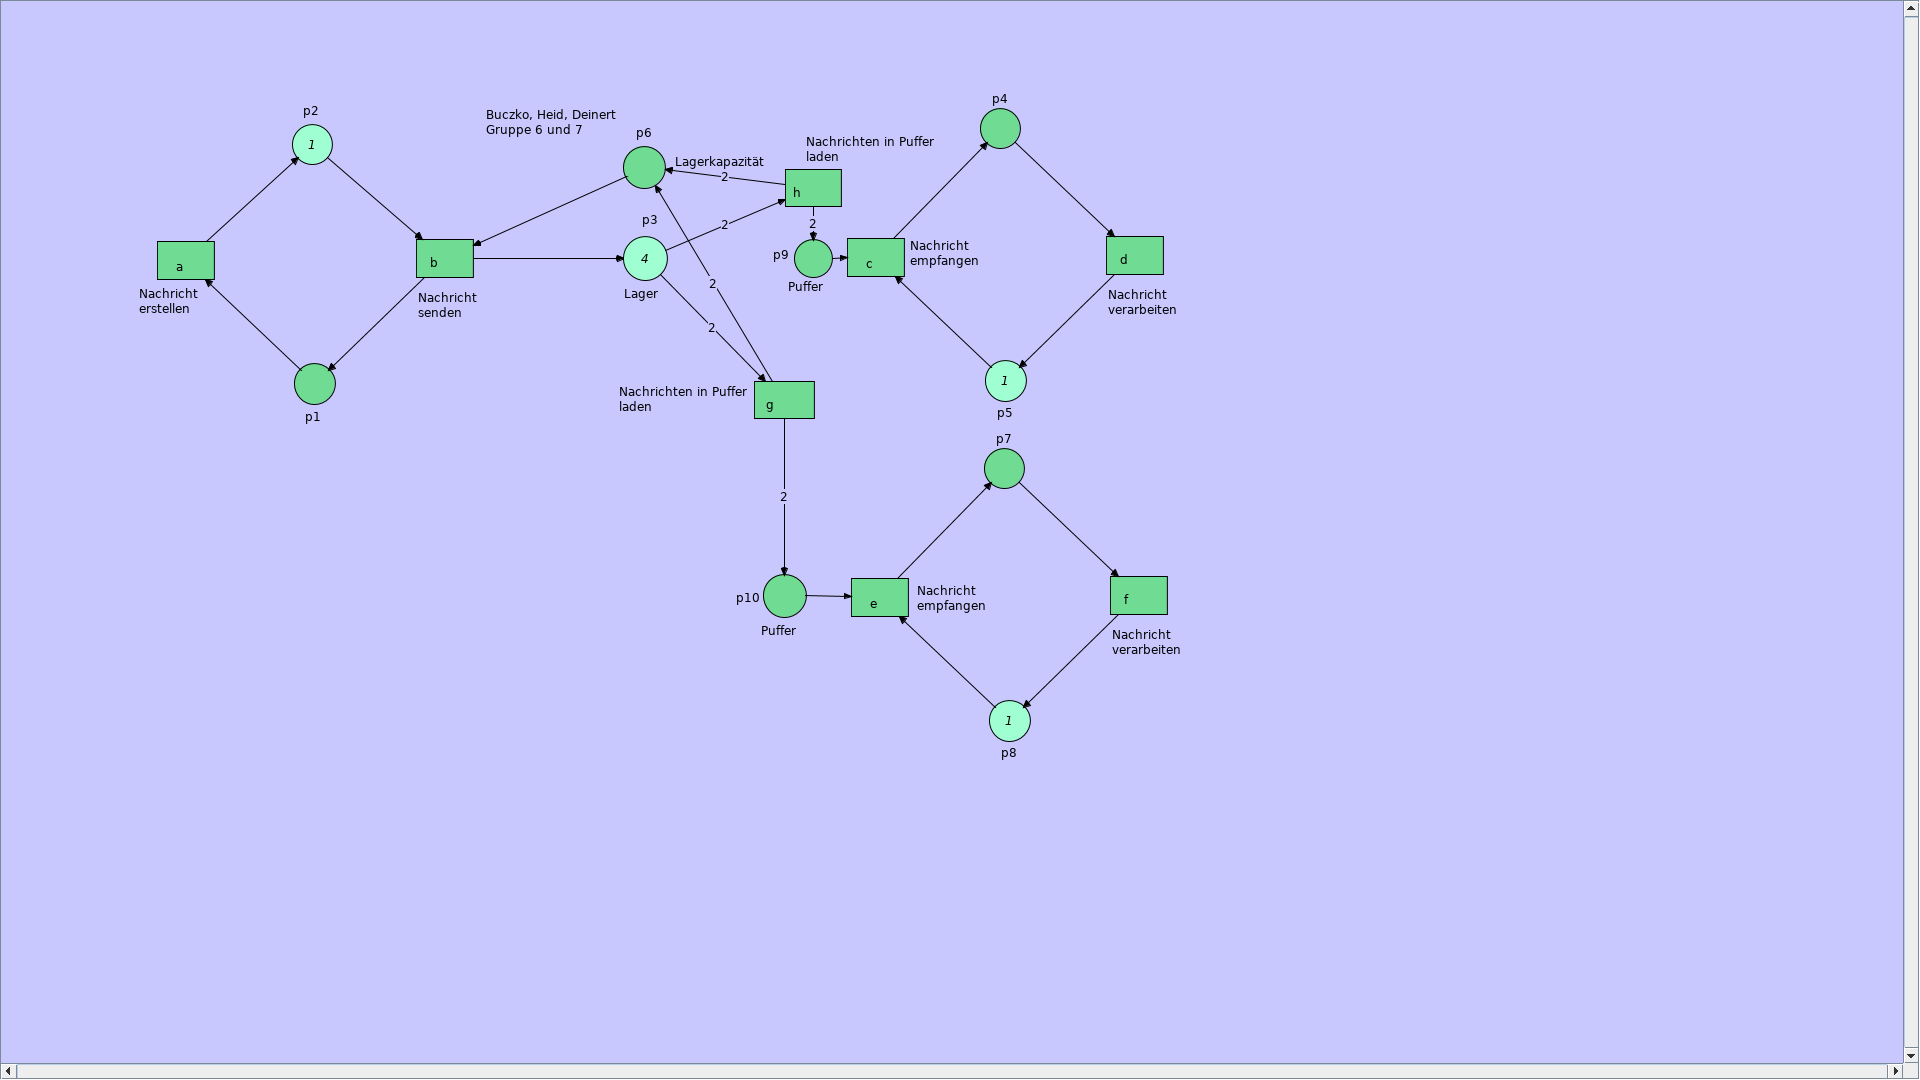
\includegraphics[scale=0.4]{6_4_5.png}
\subsection{}
\subsubsection{}
Die fett gedruckten Antworten sind die richtigen.
Ein Netzmorphismus $\phi$ ist ein Epimorphismus, falls $\phi$ bijektiv ist und für jede Kante ein Urbild existiert, d.h für alle $f_2\in F_2$ existiert ein $f_1\in F_1$ mit $\phi(f_1)=f_2$.\\
- Ja\\
\textbf{- Nein}
\subsubsection{}
Kann eine Menge Y gleichzeitig offen und abgeschlossen sein?\\
\textbf{- Ja}\\
- Nein
\subsubsection{}
Platz-berandete Mengen heißen auch ...\\
\textbf{- offen}\\
- abgeschlossen\\
- vergröbert\\
- leer
\subsubsection{}
Transitions-berandete Mengen heißen auch ...\\
- offen\\
\textbf{- abgeschlossen}\\
- vergröbert\\
- leer
\end{document}
